\chapter{Material and Methods}

\section{Data sets}
We have used four different data sets in our experiments. Three of the data sets was given by the Semeval-2013 contest. These corpora consists of a learning set, a development/evaluation set, and a test set. All sets consist of manually annotated tweets on a range of topics, including different products and events. The development set and the test set contain some overlapping tweets, so either one of these had to be used for learning and evaluation. All the data sets had more than three different target classes, e.g., 'objective', 'objective-OR-neutral'. So to make them fit a 3-way classification task, all tweets that wasn't annotated as 'positive' or 'negative' was merged into the target class 'neutral'. The distribution of target classes in the data sets are listed in Table~\ref{tab:data_sets}. None of the tweets has been pre processed or filtered in any way, so they contain hashtags, urls, emoticons etc.

\begin{table}[htb]
\centering
\begin{tabular}{|r||c|c|c|} 
\cline{2-4}
\multicolumn{1}{c|}{ } & \textbf{Learning} & \textbf{Test set 1} &\textbf{Test set 2} \\ \hline
Positive & 3270 & 526 & 368 \\ \hline
Neutral  & 4151 & 673 & 144 \\ \hline
Negative & 1288 & 313 & 176 \\ \hline
Total & 8709 & 1512 & 688 \\ \hline

\end{tabular}
\caption{These data sets was used in the experiments.}
\label{tab:data_sets}
\end{table}

In addition to the data sets that were given by (the contest), we made a small data set on our own. Before we knew about the Semeval data sets, we made a web application for manually annotation of tweets. This system was tested and used to collect a small data set, but when we got the collection of data sets from the contest we decided to cancel the collection of our own data.

Due to Twitter's privacy policy, the given data sets doesn't contain the tweet text itself, but the tweet ID that can be used to download the actual text. The Twitter API has a limit on number of downloads per hour, so Semeval-2013 provided a python script that uses the tweet ID to scrape the text from Twitter.com. This script was slow, and it didn't download all the tweet texts from the tweet IDs in the data sets. To solve this we made a new download script for node.js that was both faster and more precise. The data files outputted by the script are in the same format as the provided one. The files are tab separated (.tsv formatted) with columns that contain tweet ID, user ID, target class, and tweet text.

\section{Algorithms}

describe MaxEnt, NB, SVM, Boosting/Bagging


\chapter{Architecture}
\label{sec:experimentalsetup}

This chapter defines the architecture for the generic Twitter Sentiment Analysis system, and the implemented visualization applications. Section~\ref{sec:tsaarchitecture}, describes the architecture for the API layer as well as the sentiment classifier server. Section~\ref{sec:visualization_applications}, documents how the visualization applications are implemented and how the finished product works.

\section{TSA Architecture}
\label{sec:tsaarchitecture}

This section describes the overall architecture and how the system works. First the general system will be described, and then the API Layer and classification server in turn.  

To make the system as modularized and responsive as possible, the API layer was written in Node.js and the sentiment classifier in the Python programming language. Both systems are continuously running servers. This allows multiple services to run simultaneously, both for the API layer and the classifier. The idea is to make the system horizontally scalable.

\begin{figure}[ht]
 \begin{center}
     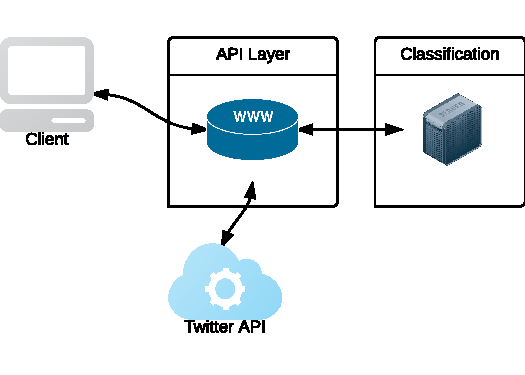
\includegraphics[width=0.8\textwidth]{../img/NetworkDiagram.pdf}
 \end{center}
 \caption[Architectural overview of the system.]{Architectural overview of the system. The client retrieves data from the Twitter API and uses the classification server for sentiment classification.}
 \label{fig:NetworkDiagram.pdf}
\end{figure}

A client makes a request to the API Layer, with the same interface as the Twitter API service. From there the API Layer will retrieve information from the Twitter API with HTTP requests, iterate over all tweets received, and send them in parallel to the classification server. When the classification server is done processing and classifying the tweet, it is sent back to the API Layer. When the API layer has received all the tweets, it responds to the client with the same JSON structure as the Twitter API sends out, only with an additional attribute noting the tweet's sentiment. This architecture and application flow can be seen in~\autoref{fig:NetworkDiagram.pdf}. 

\subsection{API Layer Extension}

To be able to have a scalable and responsive solution, the API Layer was written using the Node.js platform. Since Node.js uses JavaScript as programming language, the JSON data retrieved from the Twitter REST and Streaming API are easily manipulated and passed around. 

The API Layer works as a thin layer extending the Twitter API. This means that the interface used by Twitter, with all defined options and appropriate methods, is reflected through the API Layer. The main benefit is that all documentation for the Twitter API also documents most of this extended API Layer.

For authentication, an application is registered with a developer account at the Twitter Developer site. This creates OAuth credentials, which is used to identify the application, and to gain access to the Twitter data. For this implementation, the data is retrieved using the OAuth access for the application, not at user level. 

\subsubsection{Architectural Flow}

\begin{figure}[htb!]
 \begin{center}
     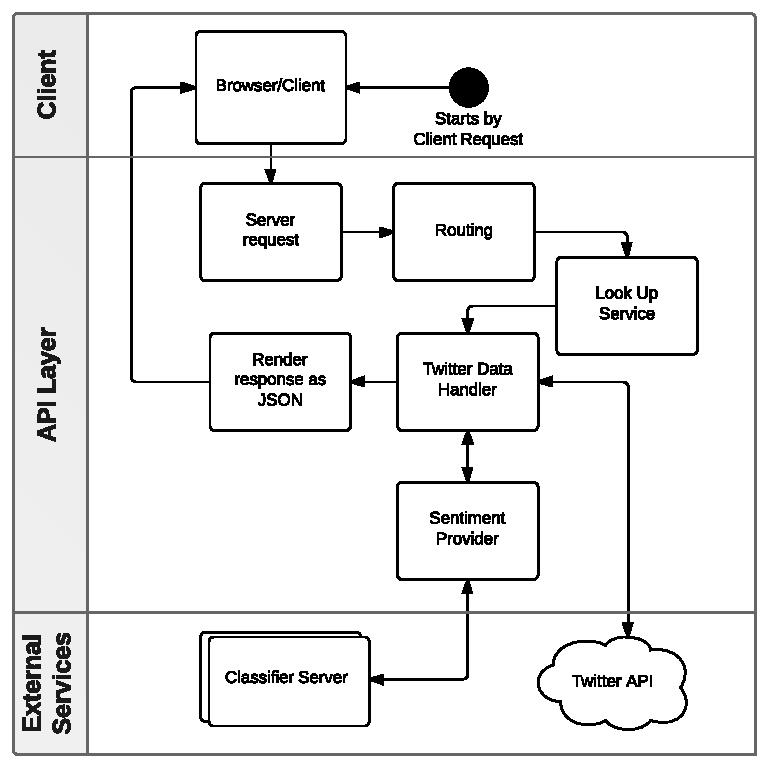
\includegraphics[width=0.8\textwidth]{../img/APILayerArcitechture.pdf}
 \end{center}
 \caption[Architectural overview of the API Layer.]{Architectural overview of the API Layer. A request is handled by the server, sending it to routing where it is processed and sent to service look-up. If a service is found, a request is sent to the Twitter API and the received data is extended by the Twitter Data Handler module to contain a sentiment. When all of the Twitter data are extended, the data is given as a response to the requesting client.}
 \label{fig:APILayerArcitechture.pdf}
\end{figure}

When a request from a client is made, the request gets processed by the server and the routing module determines what the client is looking for. When the proper service is found, the client-specified parameters are sent directly to the Twitter API, using the Twitter Data Handler module (TDH). The TDH module then iterates over all found tweets, and sends them in parallel to the classification server. When a tweet has been processed by the classification server the classified sentiment is sent back to the TBH module and the original tweet object is extended to contain a property with the sentiment. When all tweets are classified, the TBH module passes the extended twitter data to the render module. The render module renders the JSON data and sends it to the client with appropriate HTTP headers set. This application flow can be seen in~\autoref{fig:APILayerArcitechture.pdf}.

If there is an error during any part of the process, the error is caught by the routing module, and the error is rendered as a JSON object, in the same manner as it would be by the Twitter API. 

When using both the Twitter REST API and Streaming API, there is a high level of asynchronism. Especially when streaming, it is impossible to predict when the next tweet is received. Due to this the system designed needs to be able to handle this dynamic data flow. Node.js is an event-driven platform and has a natural support for asynchronous data. 

All internal and external message passing in the API Layer is asynchronous. When requesting Twitter for data, an event is triggered when that data is ready and all tweets are separately sent to the classifier. By sending all tweets separately in parallel, classification of the entire set of tweets does not take much longer than classifying only one tweet. 

When streaming, the TBH module opens a connection to the Twitter API, but never closes it. There is a continuously open connection to the Twitter server, which is feeding the TBH module with single tweets as they get stored in the Twitter system. From the first received tweet, a connection to the requesting client is opened by the render response module. This connection will also remain open. In this way there is an open connection between the client and the API Layer as well as between the API Layer and the Twitter API. The API Layer works as a middleman, taking in tweets, classifying them, and streaming them to the client. By running this entire process asynchronously, the system can process data independently of when it is published.


\subsection{Sentiment Analysis Classifier}
\label{sec:classifier_arch}

Python is computationally stronger than Node.js in many ways. Additionally, it is much more mature. There are a lot of well documented packages for handling various tasks. Scikit-learn (sklearn) is one of these packages. sklearn is package built on top of the Python packages numpy, scipy and matplotlib. sklearn integrates machine learning algorithms as SVM, NB, MaxEnt and more. sklearn implements solutions for doing feature extraction, grid searching, cross validation and a lot more for analysing text. Thus it is a good choice for the process of sentiment analysis. As a dynamic typed language, Python allows for rapid development and prototyping. These attributes are some of the reasons Python is a good fit for the present system. 

The Sentiment Analysis Classifier system runs as a server waiting for requests. The HTTP method POST is used for a client to send a \textit{stringified} tweet object to the server. Stringify is a JSON method for returning a serialized object represented by a string. The classification server converts this string to a Python dictionary. The response will be a string with the sentiment classification, that is, either \textit{positive}, \textit{neutral} or \textit{negative}. The classification scheme can be extended if necessary. 

The classifier server can be initialized with different settings for classification strategy, what port to run at, what training data to use, and whether or not to show debug data. This allows for multiple servers running at the same time, with different settings. Running multiple server instances makes it easier to compare different classification strategies. Two servers could run side by side, and a test framework could use the two servers to classify the same tweets for a comparison.

When the server is initiated, the selected model is trained by having and made availeble to be used by the classification server. 

The classification server uses a pool of child processes. For each receiving tweet, it spawns a new child from this pool and in this process the tweet is classified. This way the classification server can process several tweets in parallel, which helps the one-to-one relationship between a tweet on the classification server and the same tweet on the API Layer.

\subsubsection{Architectural Flow}

\begin{figure}[htb!]
 \begin{center}
     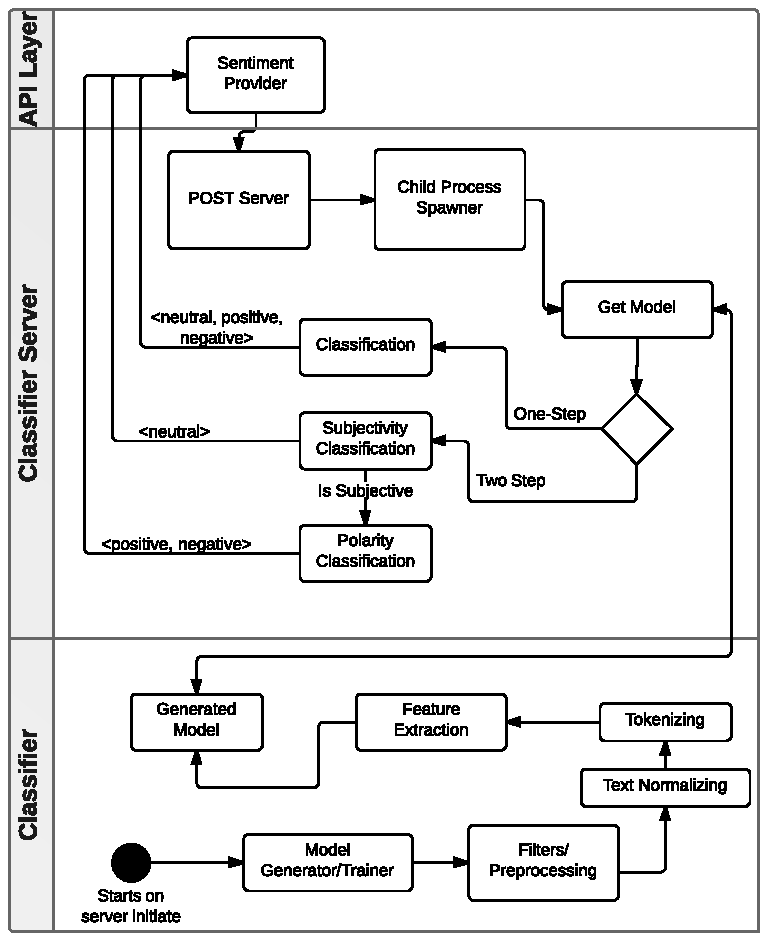
\includegraphics[width=0.8\textwidth]{../img/ClassifierArcitechture30.pdf}
 \end{center}
 \caption[Architectural overview of the classification server.]{Architectural overview of the classification server. On server start, a model for predicting seniment is generated. When a request from the API Layer is made to the POST Server, a child processes is spawned. The tweet text is extracted and sent into the model for classification. If the classification model is a one-step process, the classifier returns to the sentiment provider with either a neutral, positive or negative classification. If the generated model is two-stepped, the tweet is first classified as either neutral or subjective. If it is neutral, it is returned to the API Layer, if it is subjective, it is sent to the next step and the result from that step is returned to the sentiment provider.}
 \label{fig:ClassifierArcitechture}
\end{figure}

\begin{figure}[htb!]
 \begin{center}
     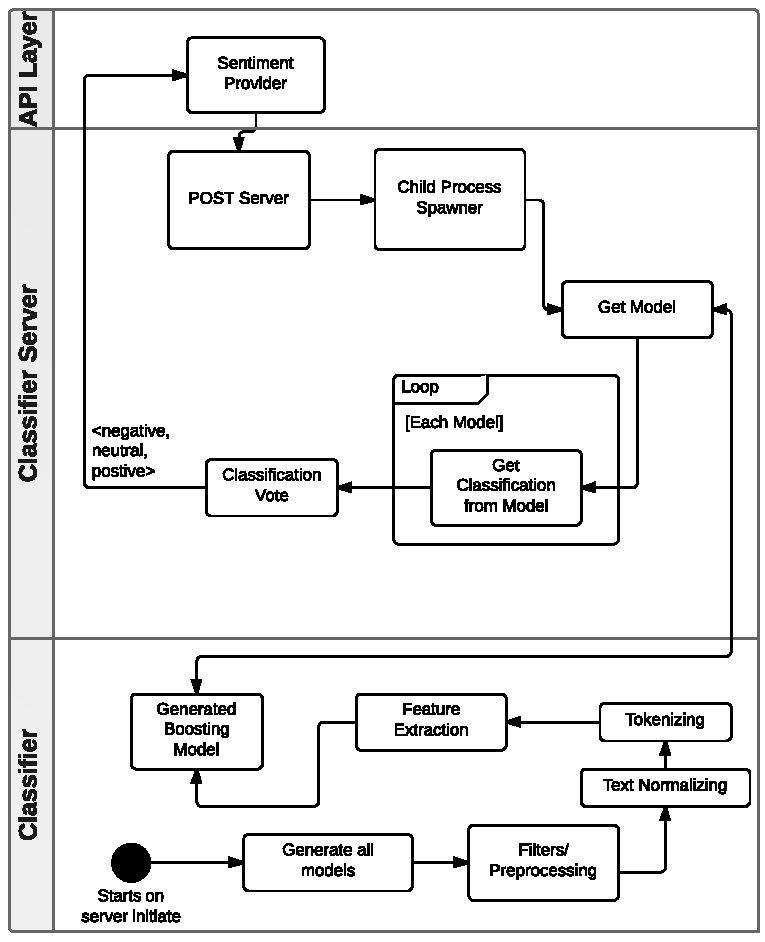
\includegraphics[width=0.8\textwidth]{../img/ClassifierArcitechture30Boosting.pdf}
 \end{center}
 \caption[Architectural overview of the classification server with Boosting.]{Architectural overview of the classification server with boosting. On server start, the Boosting model for predicting seniment is generated with a set of sub-models. When a request from the API Layer is made to the POST Server, a child processes is spawned. The tweet text is extracted and sent into the model for classification. All models predicts a sentiment and sends the sentiment to voting. For voting the Boosting model selects the sentiment with highest score and returns this to the API sentiment provider.}
 \label{fig:ClassifierArcitechtureBoosting}
\end{figure}

The Sentiment Provider module from the API Layer makes a request to the classifier's POST Server. The POST server translates the string to a Python dictionary and passes the information down to the Child Process Spawner. A new process is spawned and, using the module generated when initiating the server, the tweet is classified and returned to the API Layer.

When the classification model is trained on the server initialization, various text filters, normalizations and other pre-processing methods can be utilized, as seen in figure~\ref{fig:ClassifierArcitechture}. The model can be generated as either a one-step process, two-step process or a combination using Boosting. 

If a one-step model is used, one algorithm is used to classify the tweet as either negative, neutral or positive. If a two-step model is used, the tweet is first classified as either subjective or neutral in the subjectivity classification step. If it is neutral, the model returns with the classification. If the result is subjective, the tweet is sent to the polarity classification step, where the result can either be negative or positive. The end classification is returned to the API Layer.

When using the Boosting model, a set of sub-models is generated and all used in conjunction to predict a sentiment of a tweet. All sub-models predicts and sends the classification to a voting mechanism. The final classification is the result of the vote. This process is visualized in figure~\ref{fig:ClassifierArcitechtureBoosting}.

\subsubsection{Classification Model Structure}

The classification models are implemented by wrapping machine learning algorithms from sklearn in a inheritance based class structure. By having every model inherit from a base model, the interface is the same across every model, and the system can use the model without having knowledge what kind of algorithm it uses. An overview of this structure is presented in figure~\ref{fig:ModelsStructure}.

The base parent model implements methods for training the machine learning algorithm and for predicing either a set of documents or one document. For simple algorithms as NB, SVM and MaxEnt, these generic methods can be used, but the TwoStep and Boosting model have their own implementation. 
 
\begin{figure}[htb!]
 \begin{center}
     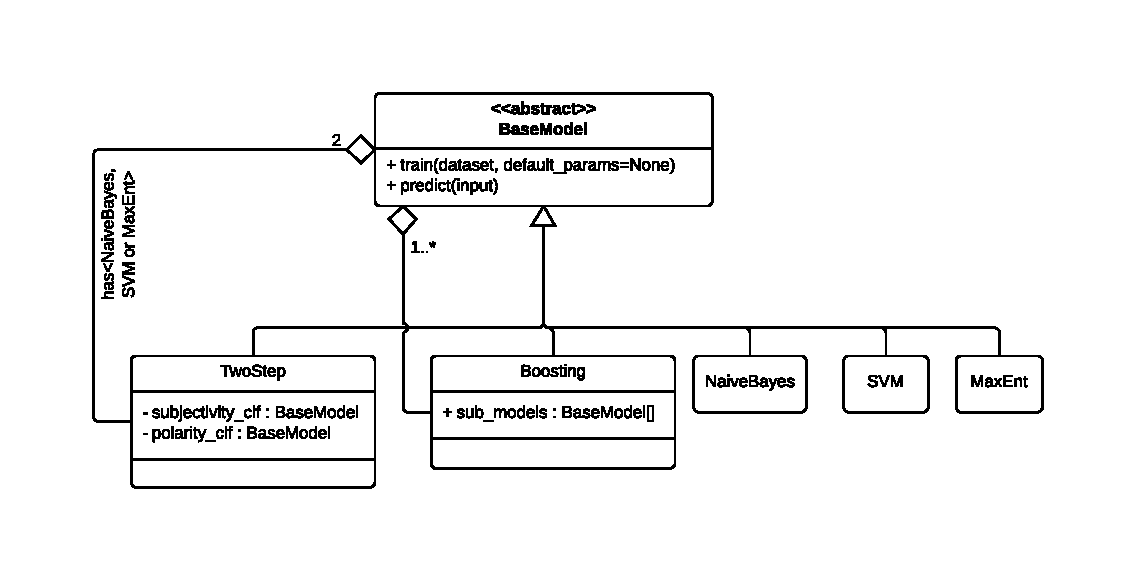
\includegraphics[width=0.8\textwidth]{../img/ModelsStructure.pdf}
 \end{center}
 \caption[Classification Model Structure Overview]{Overview of how the models are built and connected. There is a base model class implementing a method for predicting and training. All models extends from this base model. The models for NaiveBayes, SVM and MaxEnt uses the base model's implementation of train and predict, whilst the TwoStep and Boosting models implement their own. The interface for each model is the same.}
 \label{fig:ModelsStructure}
\end{figure}


\section{Visualization Applications}
\label{sec:visualization_applications}
To test and give example of how to use the generic system designed in~Section\ref{sec:tsaarchitecture}, different visualization applications were implemented. Each of these applications is described in their own sub section in this section. The sub sections are divided into describing how the applications are implemented and the finished product.

\subsection{SentiMap: Geo-location based streams}

To show how the streaming API and geo-location can be used to analyze sentiments for a location in real-time, SentiMap was developed. SentiMap is a visualization tool showing the distribution of sentiments across the states of USA with or without a search query. When a new tweet is posted, within the USA, it is used to change the colour of the state it originated from. SentiMap can show the specifics of a state, with the number of positive and negative tweets, and the total of tweets registered.

SentiMap also tracks changes in sentiment in the entire USA per second. If a major event happens, the time line would show a declining sentiment difference. The sentiment difference is calculated by taking the number of positive tweets subtracted by the number of negative tweets in a given second. 

\subsubsection{Implementation}

Most of the application is implemented on the client side, and thus running in the browser. There is a thin server side code base running, handling the stream. In this section, firstly the server will be described, and then all details about the client implementation is covered. 


\textbf{Server side implementation} \\

The client side (browser), can not connect to a Twitter stream by it self. So to be continually fed tweets in real-time, a server implementation is necessary. SentiMap's server handles the following:

\begin{enumerate}
\item Connect to the API Layer stream.
\item Open a WebSocket connection for clients to connect to. 
\item Start a HTTP server, serving HTML, JS, CSS, images and other resources. 
\item Serve the clients connected to the WebSocket with tweets.
\end{enumerate}

Since the API layer is designed as a thin layer on top of the official Twitter API, the interface is the same. This means that programming libraries designed to interact with the Twitter API, can also communicate with the API Layer. SentiMap uses a forked (branched/copied a open sourced project) Node.JS module called nTwitter\footnote{\url{https://github.com/AvianFlu/ntwitter}}. The only alteration made on nTwitter is to change the base URL for the API location from pointing to Twitters servers to instead direct to the API Layer server.

The server opens a WebSocket connection to allow clients to stream tweets from the forked nTwitter module. WebSockets\footnote{\url{http://en.wikipedia.org/wiki/WebSocket}} is a technology used to accomplish a full-duplex connection over TCP. This means that a server can push information to a client, without the client requesting it first, as with regular HTTP connection. There are two channels of communication opened for the WebSockets. One channel for streaming all tweets from the US, and one channel used to commute tweets related to a search. All clients share a connection to the non-query based stream, but for a search each client has its own connection. If there are no clients connected to the non-query based stream, the connection to the API Layer is closed, and only opened again if a client connects to the WebSocket.

The server uses a simple Node.js HTTP module to serve static file content to clients. The static content is HTML files, JavaScript libraries and code bases, images and styling files.

When a client connects to the WebSocket, on either channel, it gets fed tweets in real time. The clients receive full tweet objects directly from the API Layer. This way the clients them self can choose to do with the tweets and use them for multiple purposes at once. All logic regarding computation of sentiment statistics, graphing and logging is handled by each client.

\textbf{Client side implementation} \\

The client side uses a MV* design pattern to accomplish modularity and structure. A MV* design pattern, resembles a classical MVC pattern, but uses no controllers but instead relies more on views to handle the logic. To help with this design pattern, a JavaScript framework called Backbone.js\footnote{\url{http://backbonejs.org/}} is used. In later years Backbone has become a very popular framework to use on the client side for achieving structure in large scale applications. Backbone is a small framework and works in smaller applications as well as big corporate ones.

Every application function is its own independent module, and as such is pluggable. To support this modularity, the code is be separated into three different code structures:

\begin{enumerate}
\item Models
\item Collections
\item Views
\end{enumerate}

Models holds values and operations to interact with these values. For the SentiMap application, there are three different models; $State$, $TimelineStats$, and $TweetCount$. 

The $TimelineStats$ model holds a two dimensional array with time stamps and sentiment difference as value, and an operation to append attributes to this value. When a set of time stamp and sentiment difference is added to the array, the model announces this change to the rest of the application, to any arbitrary listeners, by using \textit{events}. 

The $TweetCount$ model operates the same as $TimelineStats$, but instead of having an array as a value, it simply stores an integer. $TweetCount$ offers operations to increase by one or reset the integer. When the integer is changed, the model announces so through events. Both the $TimelineStats$ and $TweetCount$ models are only intended to be initiated once, unlike the $State$ model.

For each state in the USA, an object is created from the $State$ model. This model holds values for state ID (nave abbreviation. e.g. NY for New York), number of positive and negative tweets for the given state. The model has operations for increasing both the negative and positive counter values by one. The model triggers an event when the values change. 

A collection is simply a collection of models. In the SentiMap applications, the only collection is states which holds all the state model objects. Collections offers operations for fetching objects based on ID. This way, a collection can retrieve the model object for New York, based on the abbreviated name. 

Views handles most of the logic and interactions with the end user. A view can represent a model or collection, but does not require to do so. A view is coupled with a HTML element in the DOM and can be used to render the contents of a model or collection of models into this DOM structure. A view can be looked at as a pluggable module. SentiMap consists of several views. Below is a list of the essential ones and a description of the view's role in the system.

\begin{description}
\item[App] \hfill \\
The App view is the heart of the application. It loads and initiates all modules (views). When App is initiated, the map, timeline, tweet counter and stream view is initiated as well. The App view has an operation (method) for switching between a query based stream (search) or non-query based.

\item[PublicStreamView] \hfill \\

The PublicStreamView and SearchView is strongly related. PublicStreamView handles the streaming of tweets when no search query is defined. PublicStreamView connects to the non-query based channel of the servers WebSocket, and attaches an operation to respond when the server pushes a new tweet. This response operation reads the tweet and based on the tweet location property, determines what state the tweet originates from. Using the ID for the state, the state model object is fetched from the state collection. Depending on whether the sentiment classification of the tweet is positive or negative, the response operation triggers the increase negative or positive tweet method on the model.

The PublicStreamView module also has methods for disconnecting from the server WebSocket, and removing the generated HTML view from the DOM.

The response handler broadcasts a global event each time a new tweet is received. 

\item[SearchView] \hfill \\

The SearchView works almost exactly the same way as the PublicStreamView. If the App triggers a change between modes (from non-query based, to search), the SearchView connects to the search channel on the WebSocket and communicates on which query it would like to receive tweets related to. The SearchView and PublicStreamView shares the response handler on a new tweet.

\item[MapView] \hfill \\

To render out a map of the USA and connect each state with a view, the MapView is initiated. The MapView is the view of the states collection. When initiated, the MapView renders out a map of the USA consisting of individual parts for each state. MapView creates a StateView object per state in the map and attributes these objects with their corresponding state models.

\item[StateView] \hfill \\

A state view is created by the MapView, and has two attribute values; a state HTML object from the map, and the state model object. 

On initialization, the StateView listens for any events on the attached model. If a state model changes its polarity (either positive or negative values are increased or reset), two operations get triggered; change colour on the map for the given state, and if the state specific statistics is visible, update the statistics.

The state view also handles the presentation of the state specific statistics. If a state on the map is clicked, the StateView of that state hides the current detailed statistics (if any), and shows the statistics for the clicked state. Before showing the chart, it makes sure that the details are up to date. 

\item[TweetCountView] \hfill \\

The TweetCountView is a simple view, initiated by the App view. On initialization, the TweetCountView attaches a view render operation on the new tweet event broadcasted by the public stream and search stream response handlers. This view renderer updates a counter on the site, informing the end user on how many tweets the SentiMap as registered on the current map. 

\item[TimelineStatsView] \hfill \\

The TimelineStatsView is initiated from the App view, and has the $TimelineStats$ model attached to it. The TimelineStatsView renders an empty graph when it is initialized. When new sentiment difference data is pushed to the attached model, the generated graph is updated to reflect these changes. The TimelineStatsView graph is updated every second. 

\end{description}

\subsubsection{Working Product}

\begin{figure}[htb!]
\begin{center}
 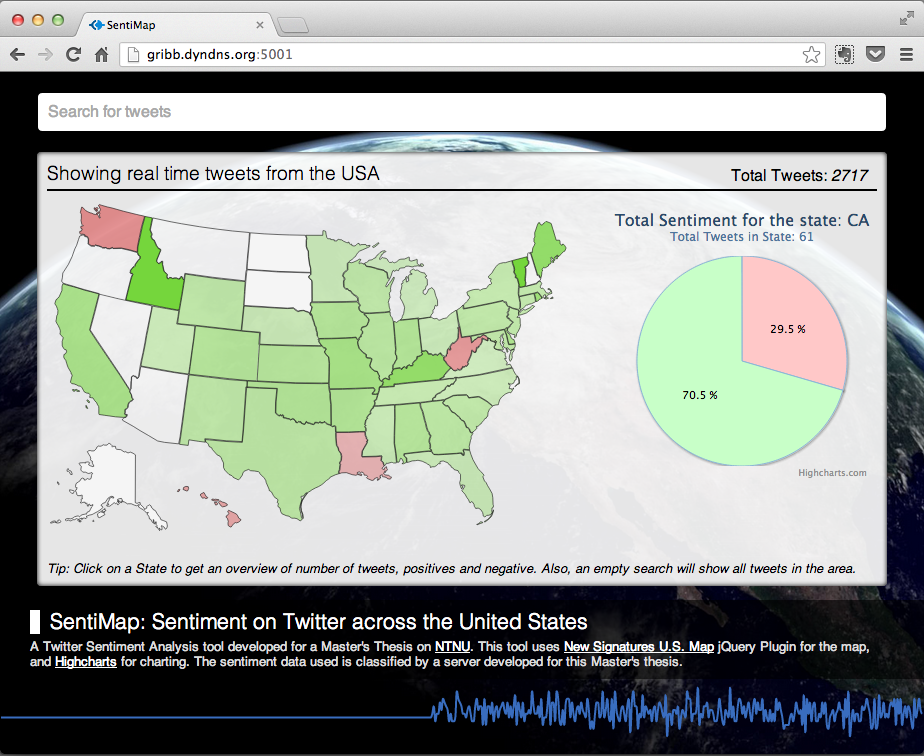
\includegraphics[width=0.8\textwidth]{../img/sentimap_screenshot.png}
 \caption{Screen shot of the SentiMap system running.}
 \label{fig:sentimap_screenshot}
\end{center}
\end{figure}

The SentiMap applications consists of three main components; an input box for search, a map of the USA with an optional details view and a timeline graph (see Figure \ref{fig:sentimap_screenshot}). Per default, the search box, is empty which results in the map being updated with tweets without any constraints regarding topic or query. If a query is typed into the search box and the return key is pressed, the map view cleared for any colour and statistics, and the map is updated with sentiments from tweets related to the submitted query (see Figure~\ref{fig:sentimap_screenshot_search}). 

\begin{figure}[htb!]
\begin{center}
 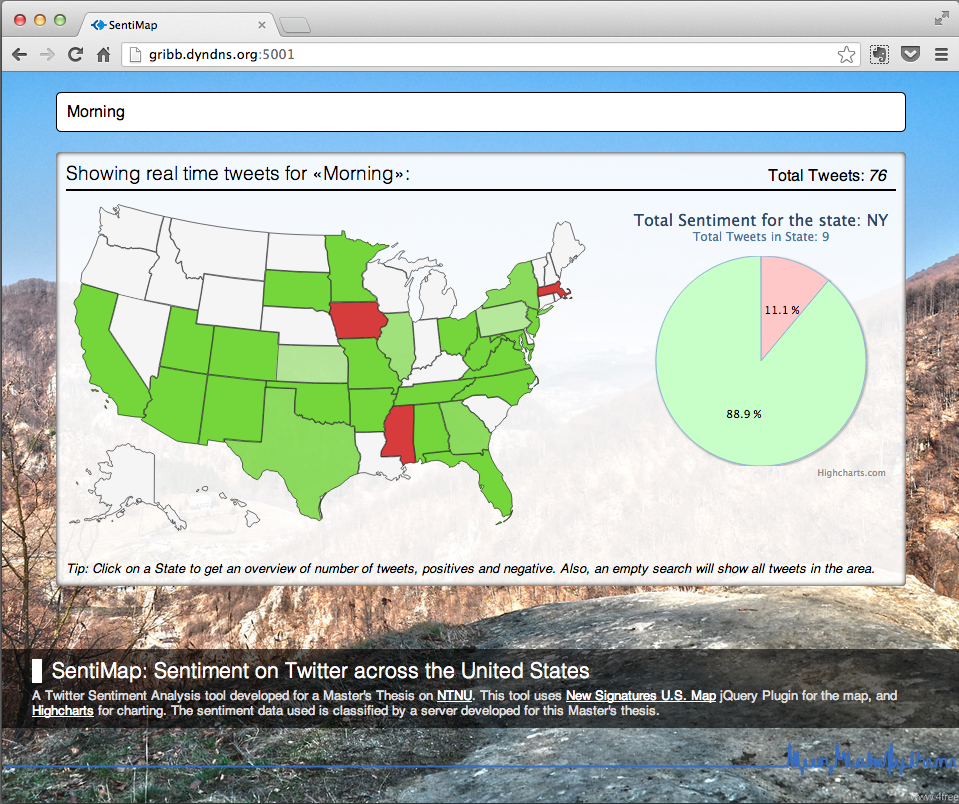
\includegraphics[width=0.8\textwidth]{../img/sentimap_screenshot_search.png}
 \caption{Screen shot of the SentiMap when searching for a query.}
 \label{fig:sentimap_screenshot_search}
\end{center}
\end{figure}

When a tweet is received, the state from where the tweet has its origin updates its colour, to reflect the change in sentiment based on the classification of that given tweet. A state where there are only negative tweets has a deep red colour, and a state with only positive tweets is clear green. If there is the same amount of positive and negative tweets, the colour of the state will be light grey. For more positive or negative a state is, the more deeper is the colour of the state. I.e. if a state is 55\% positive it is filled light green, and if a positive tweet from that state is registered, the state colour changes to a slightly more darker green.

By default, no details from a specific state is shown. But if a user clicks on a state, a pie chart is added to the right of the U.S. map. This pie chart shows the details of sentiment on a given state, and the total of tweets registered from that state. This pie chart also updates in real time.

The timeline graph on the bottom on the page, reflects the sentiment difference over time in the entire U.S.. This graph is updated every second, so if the on that second there is registered 18 positive tweets and 12 negative tweets, the graph will show the value 6. If there are no tweets registered for a given time, the graph shows the value 0. Hovering over a point on the x-axis of the graph will show the details of that value, as seen in~Figure~\ref{fig:sentimap_screenshot_timeline}.

\begin{figure}[htb!]
\begin{center}
 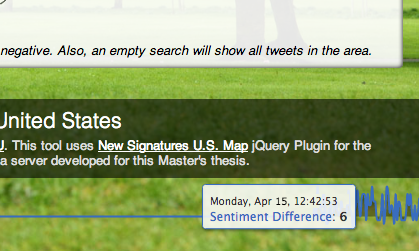
\includegraphics[width=0.6\textwidth]{../img/sentimap_screenshot_timeline.png}
 \caption[SentiMap timeline screen shot]{Showing the sentiment difference (positive minus negative sentiments) on that exact second from the streamed data.}
 \label{fig:sentimap_screenshot_timeline}
\end{center}
\end{figure}

The SentiMap always starts from scratch on initialize. So refreshing the page or when opening it for the first time, the map has no values and the time line is set to nil. All statistics and colours reflects sentiments from the second a user initializes the application.

As the SentiMap application is designed to be open over a long period of time, the background image of the application changes to a random nature photography every 30 seconds. This to give an extra visual stimuli and to make the application prettier.



\subsection{Tweet Searching}

The Twitter search API is another popular service that allows for developers to search the Twitter corpus for recent tweets on a given keyword or topic. To show how to use this search API with our classification server, a demonstration application called SentiGraph, was developed. SentiGraph consist of a chart and a Twitter timeline that shows the sentiment for each of the tweets in the chart. The chart is a combination of a pie chart, and a bar chart, where both are divided into positive, neutral and negative tweets. The sentiment of the tweets is indicated with red (negative), blue (neutral) and green (positive) colours.

\subsubsection{Implementation}

SentiGraph is a light weight web application that runs in the client's web browser. It consist of three main views: a search field, a combined chart, and a Twitter timeline. The communication between the application and the API Layer is through AJAX (Asynchronous Javasciprt and XML) technologies. AJAX is used to request and receive the response from the classification server. And by using AJAX for communication, the views can be updated with new data without reloading the entire application.

The tweets shown in the timeline includes the tweet text, its date, the author's profile picture and the sentiment classification. All these data are extracted from the tweet JSON object provided by the API layer.

The application uses CSS for responsiveness, so it fits different screen sizes. On large screens and resolutions, the presentation is divided into two columns, but when the browser window are minimized to below 1080 pixels, the timeline in the right column is moved to the left, so it appears below the chart view.

\begin{figure}[htb!]
\begin{center}
 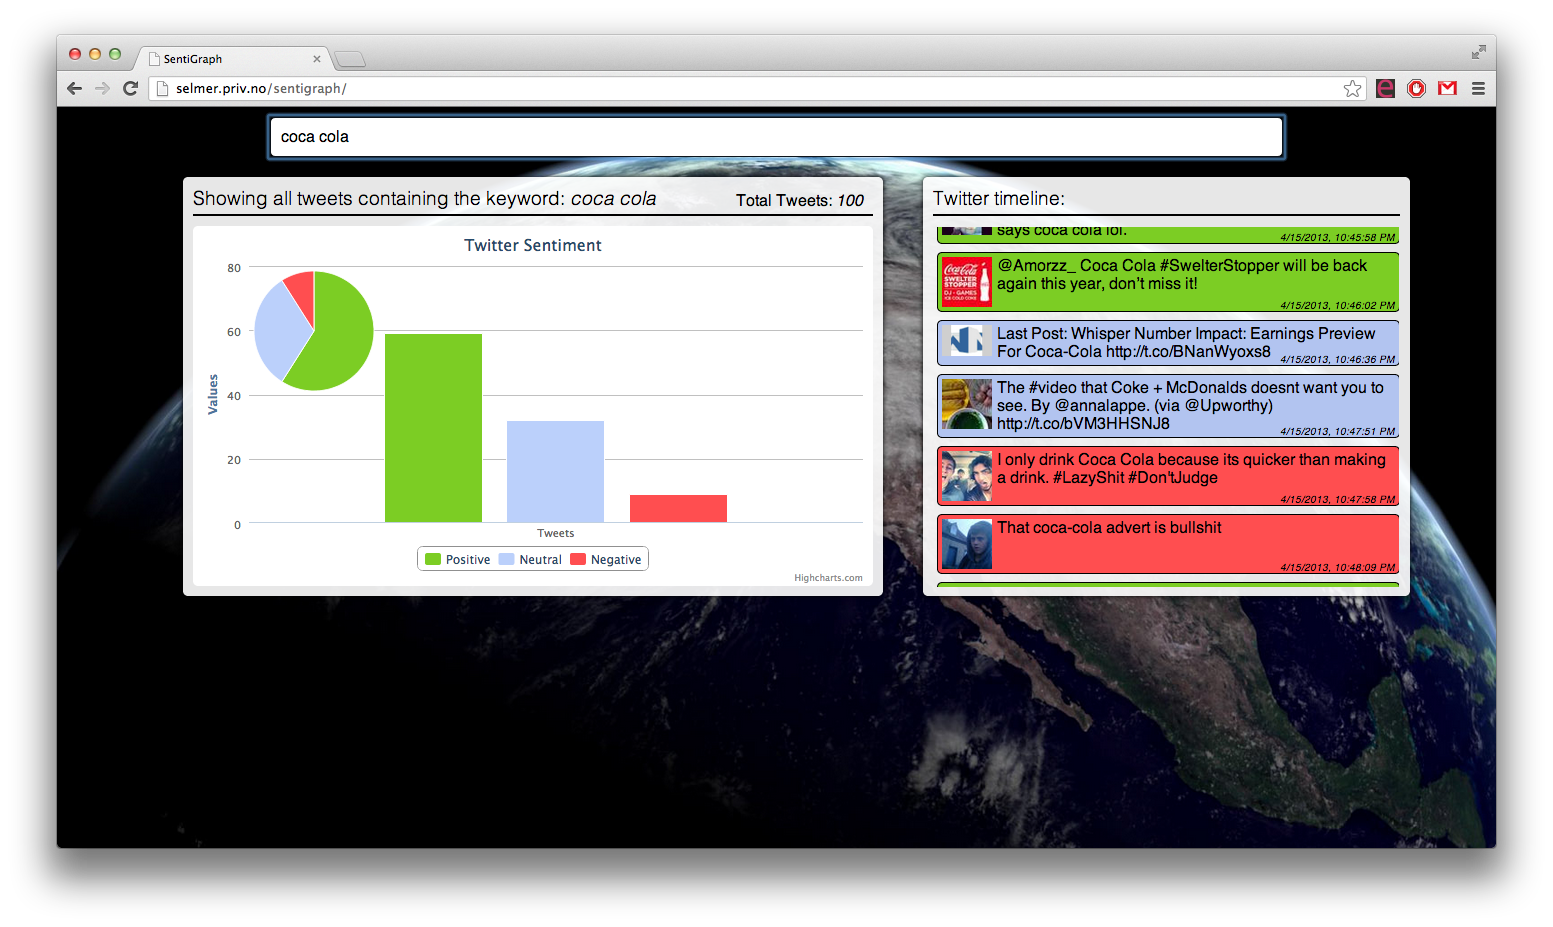
\includegraphics[width=0.8\textwidth]{../img/sentigraph_screenshot.png}
 \caption[SentiGraph screen shot]{Caption here..}
 \label{fig:sentigraph_screenshot}
\end{center}
\end{figure}

\subsubsection{Working Product}

SentiGraph allows the user to define a search query and a maximum tweet count to limit the search. The tweets returned by the API are processed in JavaScript, and for the timeline view, each tweet's HTML container element are given a CSS colour code to indicate its sentiment. In addition to colouring the container, the script also inserts the author's profile picture, and the date and time the tweet was published. The script waits for all data in each tweet container to be completely downloaded before it renders it. This is mainly to avoid collapsing HTML elements because of missing data.


